\section{Introduction}
Ephemeral Diffie-Hellman Over COSE (EDHOC) is authenticated key exchange protocol
which is designed for low-power devices in the IoT. This kind of communicating
environment requires highly restricted bandwidth as well as limited power consumption,
leading to the priorities of small message size and high-efficiency resource consumption.
In addition, given the significantly increasing number of IoT devices, security is
an important concern.

Given the foreseeable threat of Cryptographically Relevant Quantum Computer (CRQC), any
cryptographic schemes based on the hardness of integer factoring, e.g. RSA, or
discrete logarithm, e.g. Diffie-Hellman, are breakable, leading to ``Harvest Now, Decrypt Later''
attack strategy~\cite{crqc,eu-quantum-migration}. Not being out of this threat, EDHOC relies on the security of Diffie-Hellman
model, which is not quantum-resistant. Though
EDHOC was designed with post-quantum cryptography (PQC) considerations, there have not been any corresponding
specifications regarding this migration, which is stated in the Section 9.4 of RFC 9528~\cite{edhoc-rfc}:
\begin{displayquote}
    ``
    EDHOC supports all signature algorithms defined by COSE, including PQC signature algorithms such as HSS-LMS\@.
    EDHOC is currently only specified for use with key exchange algorithms of type ECDH curves, but any Key
    Encapsulation Method (KEM), including PQC KEMs, can be used in method 0. While the key exchange in method 0
    is specified with the terms of the Diffie-Hellman protocol, the key exchange adheres to a KEM interface:
    G\_X is then the public key of the Initiator, G\_Y is the encapsulation, and G\_XY is the shared secret.
    Use of PQC KEMs to replace static DH authentication would likely require a specification updating EDHOC
    with new methods.
    ''
\end{displayquote}

Furthermore, among totally 4 authentication methods (\autoref{tab:edhoc-methods}), only
the first method, which requires
rounds of interactivity, is seemingly able to be migrated to PQC through the Key Encapsulation
Mechanism (KEM) adaptation. KEM replacement to DH is a straight-forward PQC-migration strategy that
has been well-studied in widely-deployed secure protocols and frameworks, such as TLS
~\cite{optls,kemtls}, WireGuard~\cite{pqc-wireguard}, Noise~\cite{pqc-noise}, and Split-Key STS
~\cite{split-keys-sts}. However, when authentication methods based on static DH keys are utilized in EDHOC, this KEM-based
approach is doomed to fail; this issue is even raised by John Mattsson, one of the authors of EDHOC
~\cite{nike-group-discussion,edhoc-security-overview}. In those static-DH-key-based settings, a
non-interactive key exchange (NIKE) protocol is needed, which is somehow reflected
in \href{https://groups.google.com/a/list.nist.gov/g/pqc-forum/c/y_nQ3xMDRy8/m/uI1nU5iuAAAJ}{this dicussion}
among researchers.
Regarding this, CTIDH~\cite{ctidh}
and SWOOSH~\cite{swoosh}, which are isogeny-based and lattice-based respectively,
appear to be only two post-quantum NIKE currently. As presented in~\autoref{fig:swoosh-comparison},
the key size of SWOOSH is prohibitively large, which is unacceptable in constrained
environments. On the other hand, CTIDH shows an impressively small key, though its
computational time of the shared key is around 50 times slower than that of
Passive-SWOOSH\@. Given the polarized advantages and disadvantages of CTIDH
and SWOOSH along with the priority of minimal message size stated in~\cite{edhoc-rfc},
it seems that CTIDH is a more suitable choice for communicating
settings where EDHOC is deployed due to its compact key size. Furthermore, a faster and
deterministic version of CTIDH, namely dCTIDH~\cite{dctidh}, recently sheds a light
to the potentiality of ECDH replacement in certain applications.

\begin{figure}
    \centering
    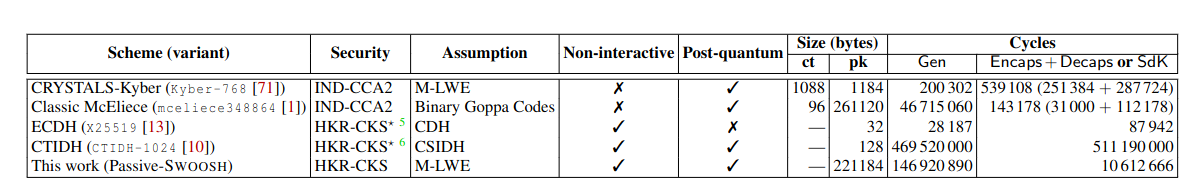
\includegraphics[height=\textheight,width=\textwidth,keepaspectratio]{kem_nike_comparision_table.png}
    \caption{Comparison of select post-quantum KEMs and NIKEs\cite{swoosh}.}
    \label{fig:swoosh-comparison}
\end{figure}

This project aims for migrating EDHOC to PQC in all authentication methods; in
other words, designing, implementing, and testing post-quantum variants of EDHOC
with all authentication methods.
While KEM-based migration is straight-forward for the first authentication method,
a PQC NIKE comes as a drop-in replacement of ECDH in the remaining methods.
Additionally, we plan to implement EDHOC protocol under the support of
Trusted Execution Environment (TEE) which ensures that secret key materials and
sensitive cryptographic services are stored and executed in a secure manner.

The proposal is structured as follows. \Cref{sec:background} introduces
premilinaries and technical background. Particular research questions and research methods are presented
in \Cref{sec:research-questions} and \Cref{sec:research-methods}, respectively.
\Cref{sec:experiment-setups} describes how to conduct experimental settings.

\section{Background}\label{sec:background}
% \subsection{CBOR}
% The Concise Binary Object Representation (CBOR) is a data format, binary representation
% of structured data, whose design objectives consists of minimal size in terms of
% code and message, and effortless extensibility. Given that the data model of CBOR is developed upon
% that of JSON, CBOR is an extended version of JSON\@. As a result, CBOR has certain properties
% that serve for the targeted devices in resource constrained environments, e.g\@. encoding
% binary data directly without base64-encoding as the medium~\cite{cbor}.

% \subsection{COSE}
% CBOR Object Signing and Encryption (COSE) specifies how basic application-layer security services, such as
% encryption, signing, and message authentication, and key encoding are performed over CBOR\@.
% In other words, COSE over CBOR acts the same role as JOSE does over JSON\@.
% Although COSE was initially designed for providing security to resource-constrained
% devices, specifically to Constrained RESTful Environments (CoRE), it is still applicable
% to other cases where one would consider using JOSE for security services~\cite{cose}.

% \subsection{CoAP}

% \subsection{OSCORE}

% EDHOC section
\subsection{EDHOC}
EDHOC is a lightweight authenticated key exchange
protocol for low-power environments such as Cellular IoT and Low-Power Radio Wide Area Network
(LoRaWAN)\@. It was especially designed to be integrated seamlessly to security framework
OSCORE, in which EDHOC provides authentication and key agreement for OSCORE-protected
communications over CoAP\@. By leveraging CBOR for object encoding and COSE for object-oriented
cryptographic operations, which are the same primitives deployed under OSCORE, EDHOC introduces
minimal extra cost. Compared to other widely-deployed authenticated key agreement protocols,
such as TLS Handshake, or
the compact version DTLS, and IKEv2, EDHOC outperforms in terms of computational
efficiency and message size while providing the equivalent security level.

\subsubsection{Overview of EDHOC}
EDHOC was built upon a variant of SIGn-and-MAc (SIGMA) family of theoretical protocols, SIGMA-I,
which is also the building block of (D) TLS Handshake and IKEv2. Specifically, EDHOC is a MAC-then-Sign
Diffie-Hellman based key exchange protocol. Two involved parties, an initiator \textit{I} and a responder
\textit{R}, are able to mutually authenticate by using their long-term public keys: public signature
key or static DH key, resulting in the 4 methods presented in \autoref{tab:edhoc-methods}.

\begin{table}
    \centering
    \begin{tabular}{|c|p{5cm}|p{5cm}|}
        \hline
        Method Type Value & Initiator Authentication Key & Responder Authentication Key\\
        \hline
        0 & Signature Key & Signature Key\\
        1 & Signature Key & Static DH Key\\
        2 & Static DH Key & Signature Key\\
        3 & Static DH Key & Static DH Key\\
        \hline
    \end{tabular}
    \caption{Authentication Keys for EDHOC Method Types~\cite{edhoc-rfc}.}
    \label{tab:edhoc-methods}
\end{table}

EDHOC includes three mandatory messages, namely
\textit{message\_1, message\_2}, and \textit{message\_3}, an optional message for providing
addtional key confirmation, \textit{message\_4},
and an error message if applicable~\cite{edhoc-rfc}. If there is no error occured, the shared
session key is established for application data protection after the \textit{message\_3}.
In general, EDHOC protocol could be described as the following steps:
\begin{itemize}
    \item \textit{message\_1}: \textit{I} sends setup information along with its identifier and
    public component of key share
    \item \textit{message\_2}: \text{R} computes the shared session key based on \textit{I}'s public component
    and its own private component. Then, \textit{R} authenticates its credential and responds
    with its own identifier,
    public credentials, all encrypted using the shared key, along with its public
    component of key share.
    \item \textit{message\_3}: \textit{I} computes the shared session key based on \textit{R}'s public component
    and its own private component. Then, \textit{I} decrypts the encrypted part of \textit{message\_2}
    and authenticates its own credentials.
    \item \textit{message\_4}: Optionally, \textit{R} explicitly confirms the shared session key.
\end{itemize}
, which is illustrated in \autoref{fig:edhoc-flow}.
After the shared secret key is exchanged, supsequent data packets are encrypted under OSCORE framework. 

\begin{figure}[h!]
    \centering
    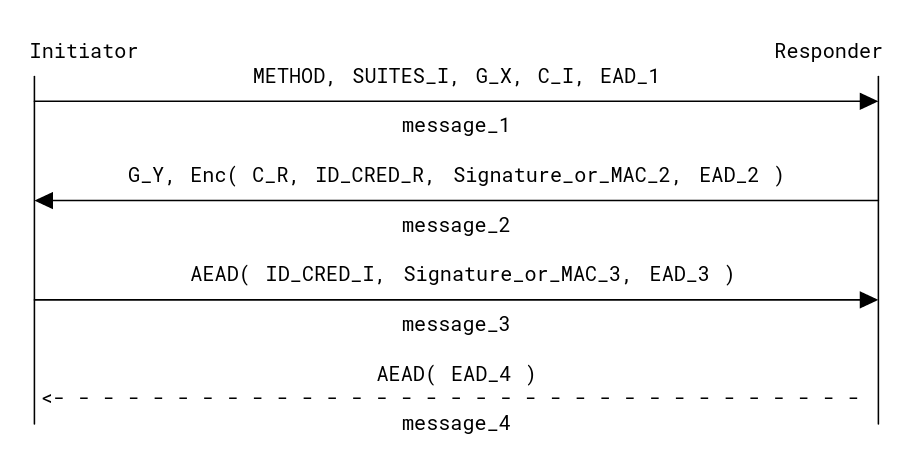
\includegraphics[height=\textheight,width=\textwidth,keepaspectratio]{edhoc-flow.png}
    \caption{EDHOC message flow (message\_4 is optional)~\cite{edhoc-rfc}.}
    \label{fig:edhoc-flow}
\end{figure}

\subsubsection{Security properties}
% Security properties to be formally verified
According to~\cite{edhoc-security-overview}, the security goals of the protocol
could be summarized as follows:
\begin{itemize}
    \item \textbf{Confidentiality}: the shared secret key at the end is only known
    to the two authenticated-communicating parties. Moreover, even if an active
    attacker compromises either one of peer's private key, they would not be able
    to compromise past session keys (Forward Secrecy).
    \item \textbf{Mutual authentication}: Each peer should re-authenticate the other
    at the end of the session, and both must agree on a new sessionidentifier, roles,
    and credentials. Critically, in the given session, the compromomise of the
    long-term secretof one party should not allow an attacker to impersonate the
    other party (Key Compromise Impersonate resistance). Furthermore, identity
    misbinding protection should be provided by the protocol.
    \item \textbf{Identity protection}: The protocol must protect one peer's identity
    from active attacks and the other peer's identity from passive attacks. Identity
    is a unique identifier which could be a cryptographic certificate, public keys, or
    MAC addresses or any other unique identifiers exchanged during the protocol.
    \item \textbf{Cryptographic strength}: The target security level of the protocol's
    key is at least 128 bits. This requirement applies to the authentication, shared
    session keys and negotiation for all cryptographic parameters.
    \item \textbf{Protection of external security data}: External Authorization Data (EAD)
    should have the same level of protection as the protocol message.
    \item \textbf{Downgrade protection}: To deal with long-term deployment,
    crytographic agility must be provided to support different cryptographic primitives,
    resulting in a mutually agreed cipher suit after a round of negotiation.
    Downgrade protection is essential to prevent
    attackers from forcing the use of weaker cryptography. This includes preventing
    cipher suite downgrade attacks (forcing less secure cipher suites) and key material
    downgrade attacks (manipulating key derivation to use weaker keys).
\end{itemize}

In order to guarantee that the protocol satisfies the aforementioned high-level security goals,
researchers have formally verified, using
both symbolic and computational models, certain drafts (12,15,17,23) of EDHOC with all authentication
methods~\cite{edhoc-sec-analysis-draft-12,edhoc-sec-analysis-draft-15,edhoc-sec-analysis-draft-17,edhoc-sec-analysis-draft-23}.
Given those security analyses, a security analysis of the proposed post-quantum variant could
be built upon them.

\subsection{Key Encapsulation Mechanism (KEM)}
A KEM is a public encryption scheme that establishes a shared secret key, which can be used
for symmetric encryption, between two communicating parties. According to~\cite{kem-definition,kem-design},
a KEM consists of three probabilistic polynomial-time (PTT) algorithms:
\begin{itemize}
    \item \textbf{KEM.KeyGen}: a probabilistic key generation algorithm that takes security parameters
    $1^\lambda$ as input and produces a public/secret key pair $(PK,SK)$
    \item \textbf{Encap}: a probabilistic key encapsulation, also known as polynomial-time
    encryption, algorithm that takes a public key $PK$ as input and produces an encapsulated
    key pair $(K,C)$, sometimes $C$ is also known as a ciphertext or an encapsulation of the
    key $K$.
    \item \textbf{Decap}: a probabilistic key decapsulation, also known as polynomial-time
    decryption, algorithm that takes a ciphertext $C$ and a secret key $SK$ as input, and
    recover the key $K$.
\end{itemize}

As a result, the secure KEM key $K$, the output of \textbf{Encap} and \textbf{Decap}, is shared
between two communicating parties.

% ML_KEM section
\subsubsection{Module-Lattice-Based Key-Encapsulation Mechanism (ML-KEM)}
At the time of writing, among several proposed KEMs, only CRYSTALS-KYBER~\cite{crystal-kyber},
whose name is later changed to ML-KEM, is standardized by NIST~\cite{FIPS203}. The security
of ML-KEM is based on the hard problem called Module Learning with Errors (MLWE)~\cite{mlwe}, which
is a more general version of the Learning With Errors (LWE)~\cite{lwe}.

% -----------------------
% TODO: more mathematical description on the LWE and MLWE could be placed here
% -----------------------

ML-KEM guarantees IND-CCA2 security~\cite{ml-kem-ind-cca,crystal-kyber}.

% SWOOSH section
% \subsection{SWOOSH}
% Non-interative key exchange (NIKE) is an authenticated key agreement protocol that
% does not require additional rounds of interation between communicating parties for
% shared key establishment. As a result, it eliminates the requirement of simultaneously
% active status among involving parties, which is suitable for messaging application, e.g.
% a receiver is offline at some point, or non-interactive authentication methods
% (1,2, and 3) in EDHOC\@.

% SWOOSH is a lattice-based NIKE, relying on the hardness of MLWE problem. In fact,
% prior to SWOOSH, lattice-based NIKE was considered impractical due to the threshold,
% theoretically proved using information theory, in constructing lattice-based NIKE
% with non-interactive reconciliations~\cite{lwe-nike-threshold}. Although SWOOSH
% does not violate the aforementioned theoretical barrier, it demonstrates that
% a lattice-based, or more specifically M-LWE-problem-based, NIKE protocol is
% still sufficiently efficient, overcoming the traditional limits~\cite{swoosh}.

% The \autoref{fig:swoosh-comparison} presents the performance of SWOOSH compared to
% that of other post-quantum and non-quantum-resistant counterparts.


% NIKE
\subsection{Non-Interative Key Exchange (NIKE)}
Following~\cite{nike-definition,nike-abstract}, NIKE is defined as a tuple of three
PPT algorithms: \textbf{Setup}, \textbf{NIKE.KeyGen}, and \textbf{SharedKey} accompanying
an identity space $IDS$ and a shared key space $SHK$.
\begin{itemize}
    \item \textbf{Setup}: a common setup algorithm that takes security parameter $1^\lambda$
    as input and outputs a set of system parameters $params$.
    \item \textbf{NIKE.KeyGen}: a key generation algorithm that takes $params$ and an identity
    $ID \in IDS$ as input and produces a public/secret key pair $(PK,SK)$.
    \item \textbf{SharedKey}: a shared key establishment algorithm that takes as input an
    identity $ID_1 \in IDS$ and a public key $pk_1$ together with another identity
    $ID_2 \in IDS$ and its corresponding secret key $sk_2$ and returns either a shared key $k \in SHK$,
    or a failure symbol $\bot$. It is assumed that \textbf{SharedKey} always outputs
    $\bot$ if $ID_1 = ID_2$
\end{itemize}

Regarding the correctness, given any pair of identities $ID_1$, $ID_2$ along with their
corresponding public/secret key pairs $(pk_1,sk_1)$ and $(pk_2, sk_2)$, the algorithm
\textbf{SharedKey} holds the following constraint:
\begin{align*}
    \textbf{SharedKey}(ID_1,pk_1,ID_2,sk_2) = \textbf{SharedKey}(ID_2,pk_2,ID_1,sk_1)
\end{align*}

% CTIDH
\subsubsection{dCTIDH}
Commutative Supersingular Isogeny Diffie-Hellman (CSIDH)~\cite{csidh} is an isogeny-based NIKE that
enables parties to establish a shared key using endomorphisms of supersingular elliptic curves.
Its security is based on the hardness of computing endomorphism rings of supersingular
elliptic curves, a problem believed to be hard even for quantum computers. However,
it introduces a high computational cost, which is especially not desired in resource-constrained
environments, due to large prime fields and group actions. In addittion, as a consequence of its probabilistic
nature, CSIDH is difficult to implement in constant-time~\cite{csidh}. To make CSIDH constant-time,
many approaches rely on dummy operations, operations that do not affect the result
depending on values in secret key, which leads to fault injection attacks
~\cite{csidh-fault-injection,csidh-fault-injection-2}. Depending on the specific use case,
this type of physical attack is considered whether problematic or not~\cite{dctidh}.

Compressed Torsion-point Isogeny Diffie-Hellman (CTIDH)~\cite{ctidh} is an optimized version of CSIDH\@.
CTIDH has solved the issues of constant-time by introducing dummy operations, therefore it is
a dummy-based implementation. By leveraging a different way of specifying the key space and
some algorithmic modifications, CTIDH, to date, is the most efficient constant-time implementation
of CSIDH in terms of both key size and computaitonal cost, even better than time-variant CSIDH\@.

dCTIDH is a deterministic version of CTIDH\@. Deterministics implementations do not require
a high-quality source of entropy during computation. The results from~\cite{dctidh} shows
that dCTIDH not only outperforms the deterministic CSIDH (dCSIDH), but also
non-deterministic CTIDH\@. At the time of writing, dCTIDH is the most efficient
constant-time, deterministic implementation.

\subsection{Trusted Execution Environment (TEE)}
TEE is a secure, tamper-resistant processing environment providing code executation,
memory and storage capabilities on a separated kernel from a rich execution
environment (REE)~\cite{tee-mobile}. It guarantees the authentication
of executed code, the integrity of runtime states, and the confidentiality of
code, data, and runtime states stored on a persistent memory~\cite{tee-overview}.
By isolating the REE, also known as the ``normal'' execution environment, from
highly secure environments so that sensitive operations and data are protected
and sandboxed inside TEE, TEE enhances the security level of sensitive services
even if they interact with a non-secure world.

In the cryptography context, TEE is a sandboxed environment that securely stores
and handles functions associated to secret key materials, preventing the leakage
of private keys.

\section{Research questions}
~\label{sec:research-questions}
\begin{itemize}
    \item Is it possible, if yes then how to integrate quantum-resistant cryptographic schemes into EDHOC
    without any major changes in its design and specification?
    \item What are trade-offs in terms of message size, cpu cycle, and latency given that
    EDHOC was designed specifically for highly restricted settings? According to EDHOC RFC~\cite{edhoc-rfc},
    minimal message size is the top priority. Moreover, in terms of time latency, the time distribution
    needs to be considered during evaluation besides the average value which could be drastically affected by
    the rarely-appeared outliers.
    \item Does the PQC-adopted design still meets security goals of the original protocol as
    well as the PQC security level standardized by NIST\@?
    % EDHOC implementation with TEE hardening.
    \item Given TEE-protected EDHOC implementation~\cite{oscore-tee-performance}, is there any
    significant overheads introduced by the PQC-variant of EDHOC\@? If yes, does the security
    enhancement provided by TEE outweight those extra costs?
\end{itemize}

\section{Research methods}
~\label{sec:research-methods}
\begin{itemize}
    \item Modifies EDHOC design to adapt KEM for the method 0, and quantum-resistant NIKE, SWOOSH or CTIDH,
    for the remaining methods.
    \item Formally verifies the PQC-variant designs, using automated tool such as ProVerif.
    \item Implements PQC-variant EDHOC in the manner of TEE isolation. Leveraging the existing work
    of \href{https://github.com/eriptic/uoscore-uedhoc}{{\textmu}OSCORE-{\textmu}EDHOC}~\cite{oscore-tee-performance},
    which is a TEE-supported implementations of the original (non-quantum-resistant) EDHOC\@.
    \item Measures the performance of PQC-variant EDHOC in terms of message size, cpu cycle,
    and latency, as well as demystify the time distribution. Additonally, compare its performance to that of DTLS, a widely used protocol in IoT
    environments, and the original (non quantum-safe) EDHOC\@.
\end{itemize}

\section{Experimental setups}
~\label{sec:experiment-setups}
Since the firmware $\mu$OSCORE-$\mu$EDHOC would be used as the baseline for the post-quantum
variant implementation, I would follow their \href{https://github.com/eriptic/uoscore-uedhoc/tree/main/samples/zephyr_edhoc}{setups}
for reproducability and comparability.

\subsection{EDHOC between two microcontrollers}
Requirements:
\begin{itemize}
    \item Zephyr OS is needed for constrained devices.
    \item Two microcontrollers (e.g.\ nRF52832, nRF52840).
    \item Two Raspberry Pi act as IPv6 over BLE routers for nrf52832.\ If nRF52840
    is utilized, there is no need for these external routing devices as nRF52840 has
    built-in BLE\@.
\end{itemize}